% !TEX root = ../thesis.tex
\section{Visual Encoding}
\label{sec:vl:gog}

The simplest Vega-Lite specification\,---\,referred to as a \emph{unit}
specification\,---\,describes a single Cartesian plot with the following
four-tuple:

\centerline{\emph{unit := (data, transforms, mark-type, encodings)}}

The \emph{data} definition identifies a data source, a relational table
consisting of records (rows) with named attributes (columns). This data table
can be subject to a set of \emph{transforms}, including filtering and adding
derived fields via formulas. The \emph{mark-type} specifies the geometric object
used to visually encode the data records. Legal values include \emph{bar},
\emph{line}, \emph{area}, \emph{text}, \emph{rule} for reference lines, and
plotting symbols (\emph{point} \& \emph{tick}). The \emph{encodings} determine
how data attributes map to the properties of visual marks. Formally, an encoding
is a seven-tuple:

\centerline{\emph{encoding := (channel, field, data-type, value, functions, scale, guide)}}

Available visual encoding \emph{channels} include spatial position (\emph{x},
\emph{y}), \emph{color}, \emph{shape}, \emph{size}, and \emph{text}. An
\emph{order} channel controls sorting of stacked elements (e.g., for stacked bar
charts and the layering order of line charts). A \emph{path} order channel
determines the sequence in which points of a line or area mark are connected to
each other. A \emph{detail} channel includes additional group-by fields in
aggregate plots.

The \emph{field} string denotes a data attribute to visualize, along with a
given \emph{data-type} (one of \emph{nominal}, \emph{ordinal}, \emph{quantitative} or
\emph{temporal}). Alternatively, one can specify a constant literal \emph{value}
to serve as the data field. The data field can be further transformed using
\emph{functions} such as binning, aggregation (e.g., mean), and sorting.

An encoding may also specify properties of a \emph{scale} that maps from the
data domain to a visual range, and a \emph{guide} (axis or legend) for
visualizing the scale. If not specified, Vega-Lite will automatically populate
default properties based on the \emph{channel} and \emph{data-type}. For \emph
{x} and \emph{y} channels, either a linear scale (for quantitative data) or an
ordinal scale (for ordinal and nominal data) is instantiated, along with an
axis. For \emph{color}, \emph{size}, and \emph{shape} channels, suitable
palettes and legends are generated. For example, quantitative color encodings
use a single-hue luminance ramp, while nominal color encodings use a categorical
palette with varied hues. Our default assignments largely follow the model of
prior systems~\cite{stolte:polaris, voyager}.

Unit specifications are capable of expressing a variety of common, useful plots
of both raw and aggregated data. Examples include bar charts, histograms, dot
plots, scatter plots, line graphs, and area graphs. Our formal definitions are
instantiated in a JSON (JavaScript Object Notation) syntax, as shown in
\cref{fig:unit1,fig:unit2,fig:unit3}.

\begin{figure}[h!]
\centering
  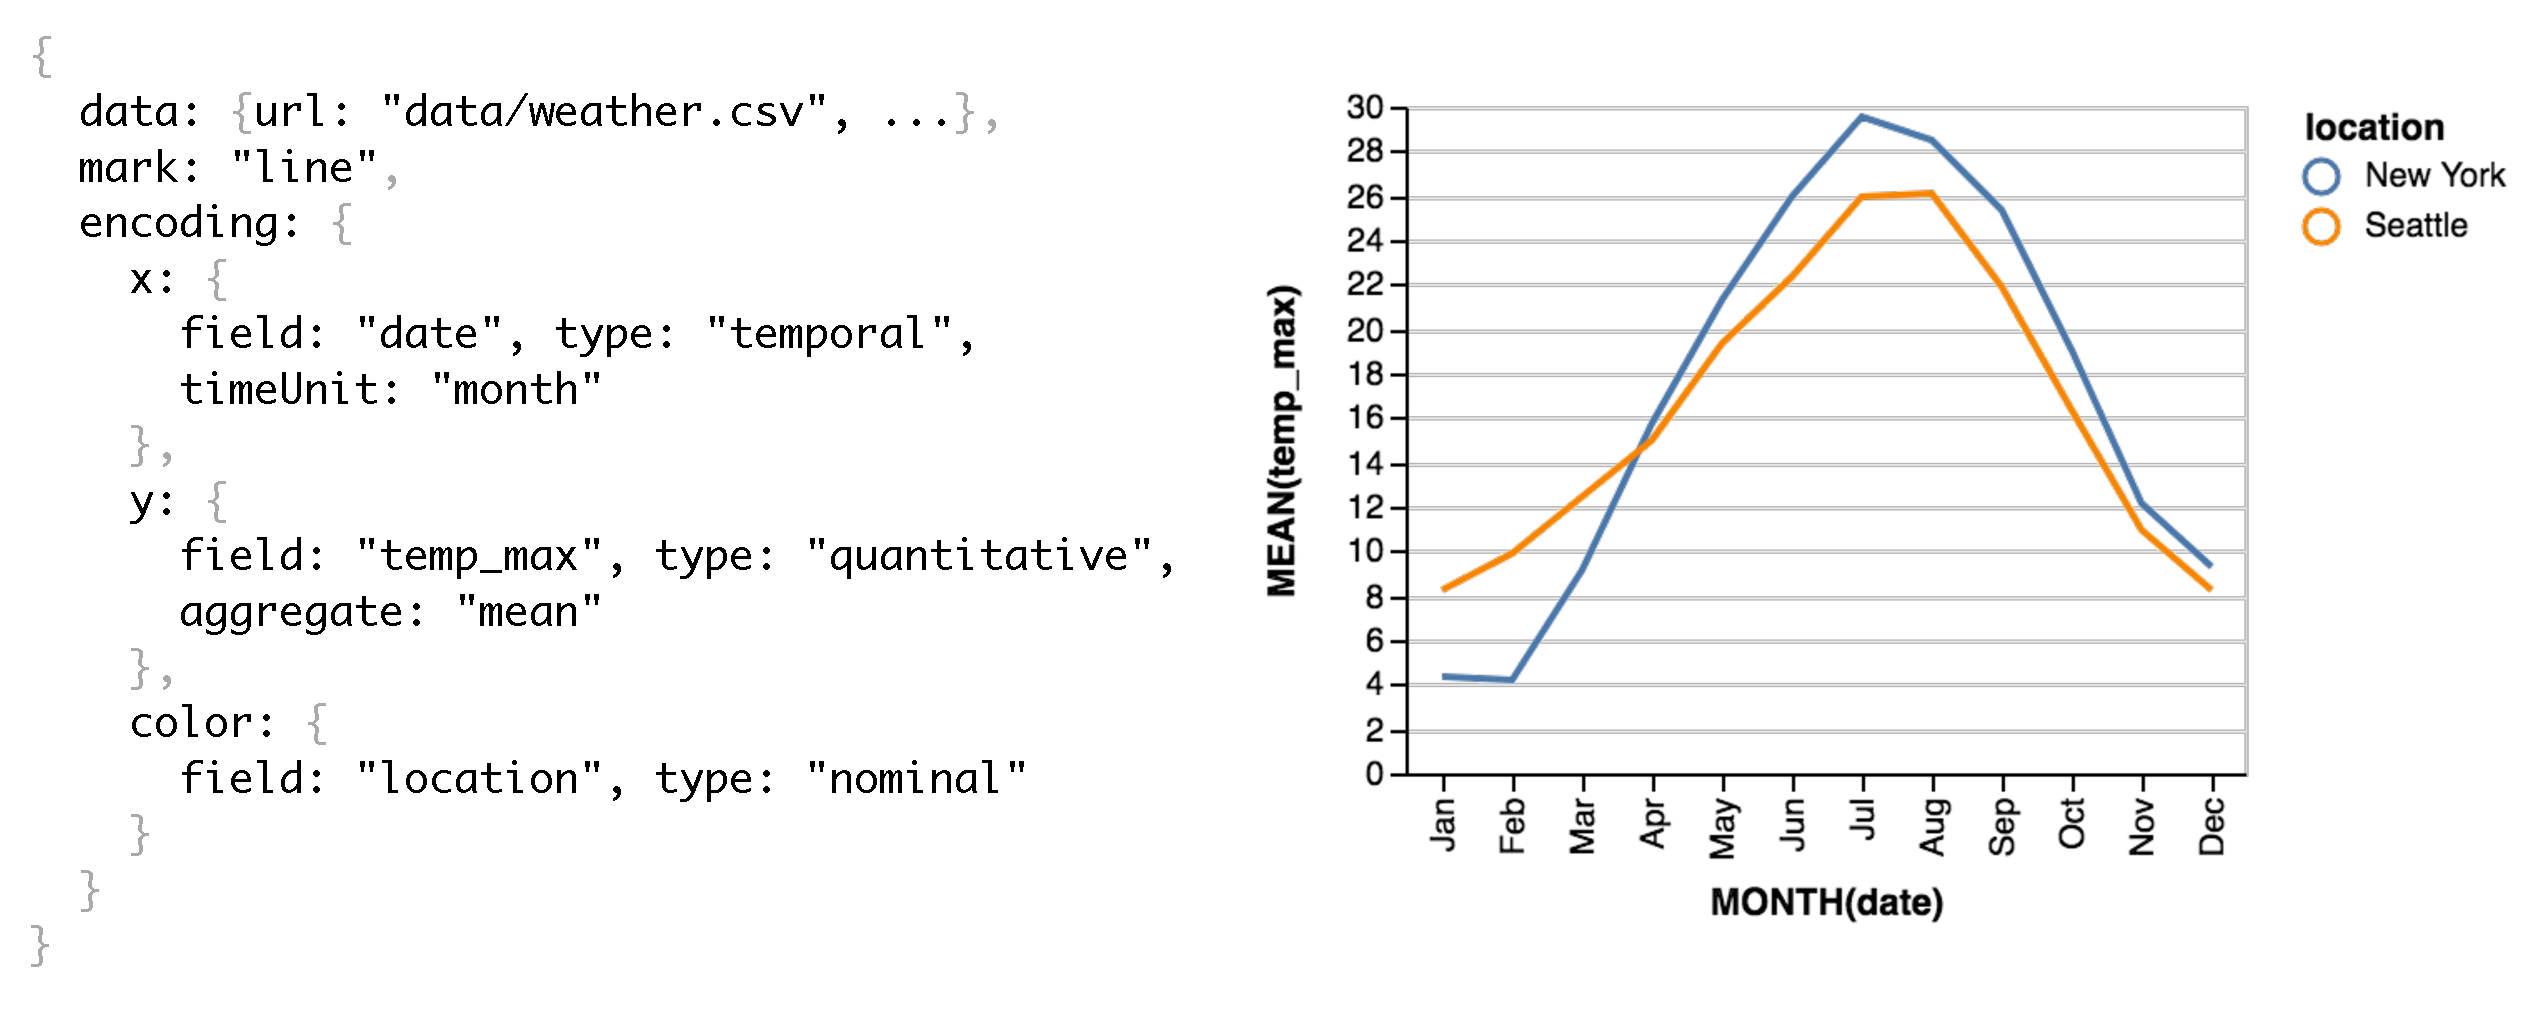
\includegraphics[width=\textwidth]{unit-1}
  \caption{A unit specification that uses a \emph{line} mark to visualize the
  \emph{mean} temperature for every \emph{month}.}
  \label{fig:unit1}
\end{figure}

\begin{figure}[h!]
  \centering
  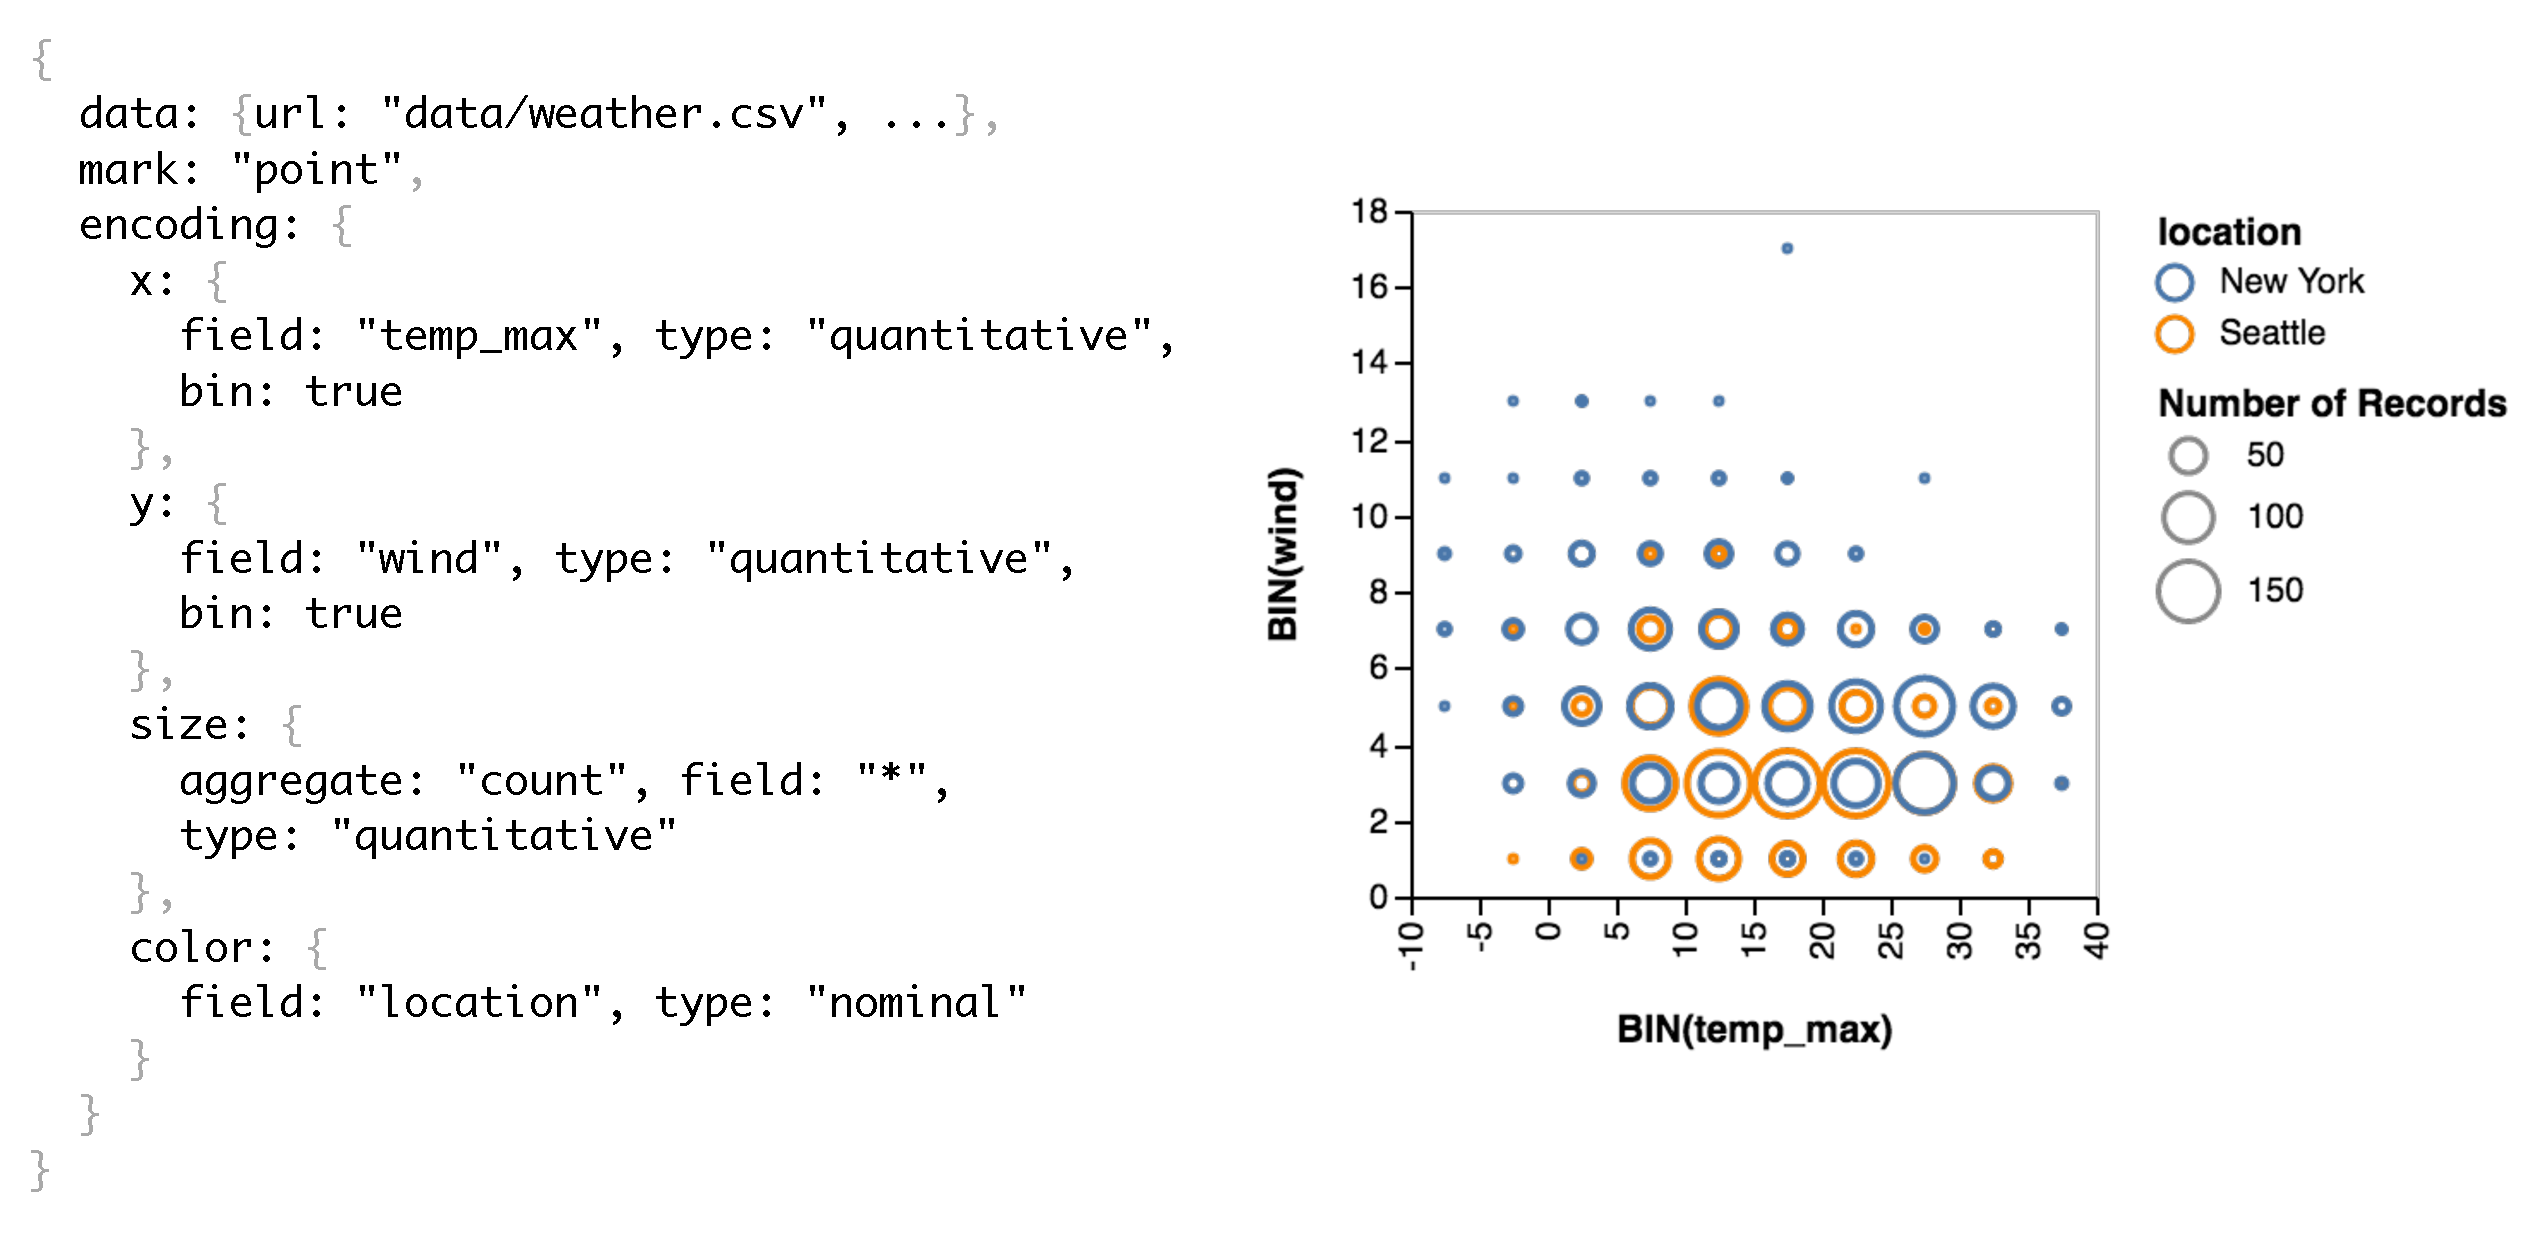
\includegraphics[width=\textwidth]{unit-2}
  \caption{A \emph{binned} scatterplot visualizes correlation between wind
  and temperature.}
  \label{fig:unit2}
\end{figure}

\begin{figure}[h!]
  \centering
  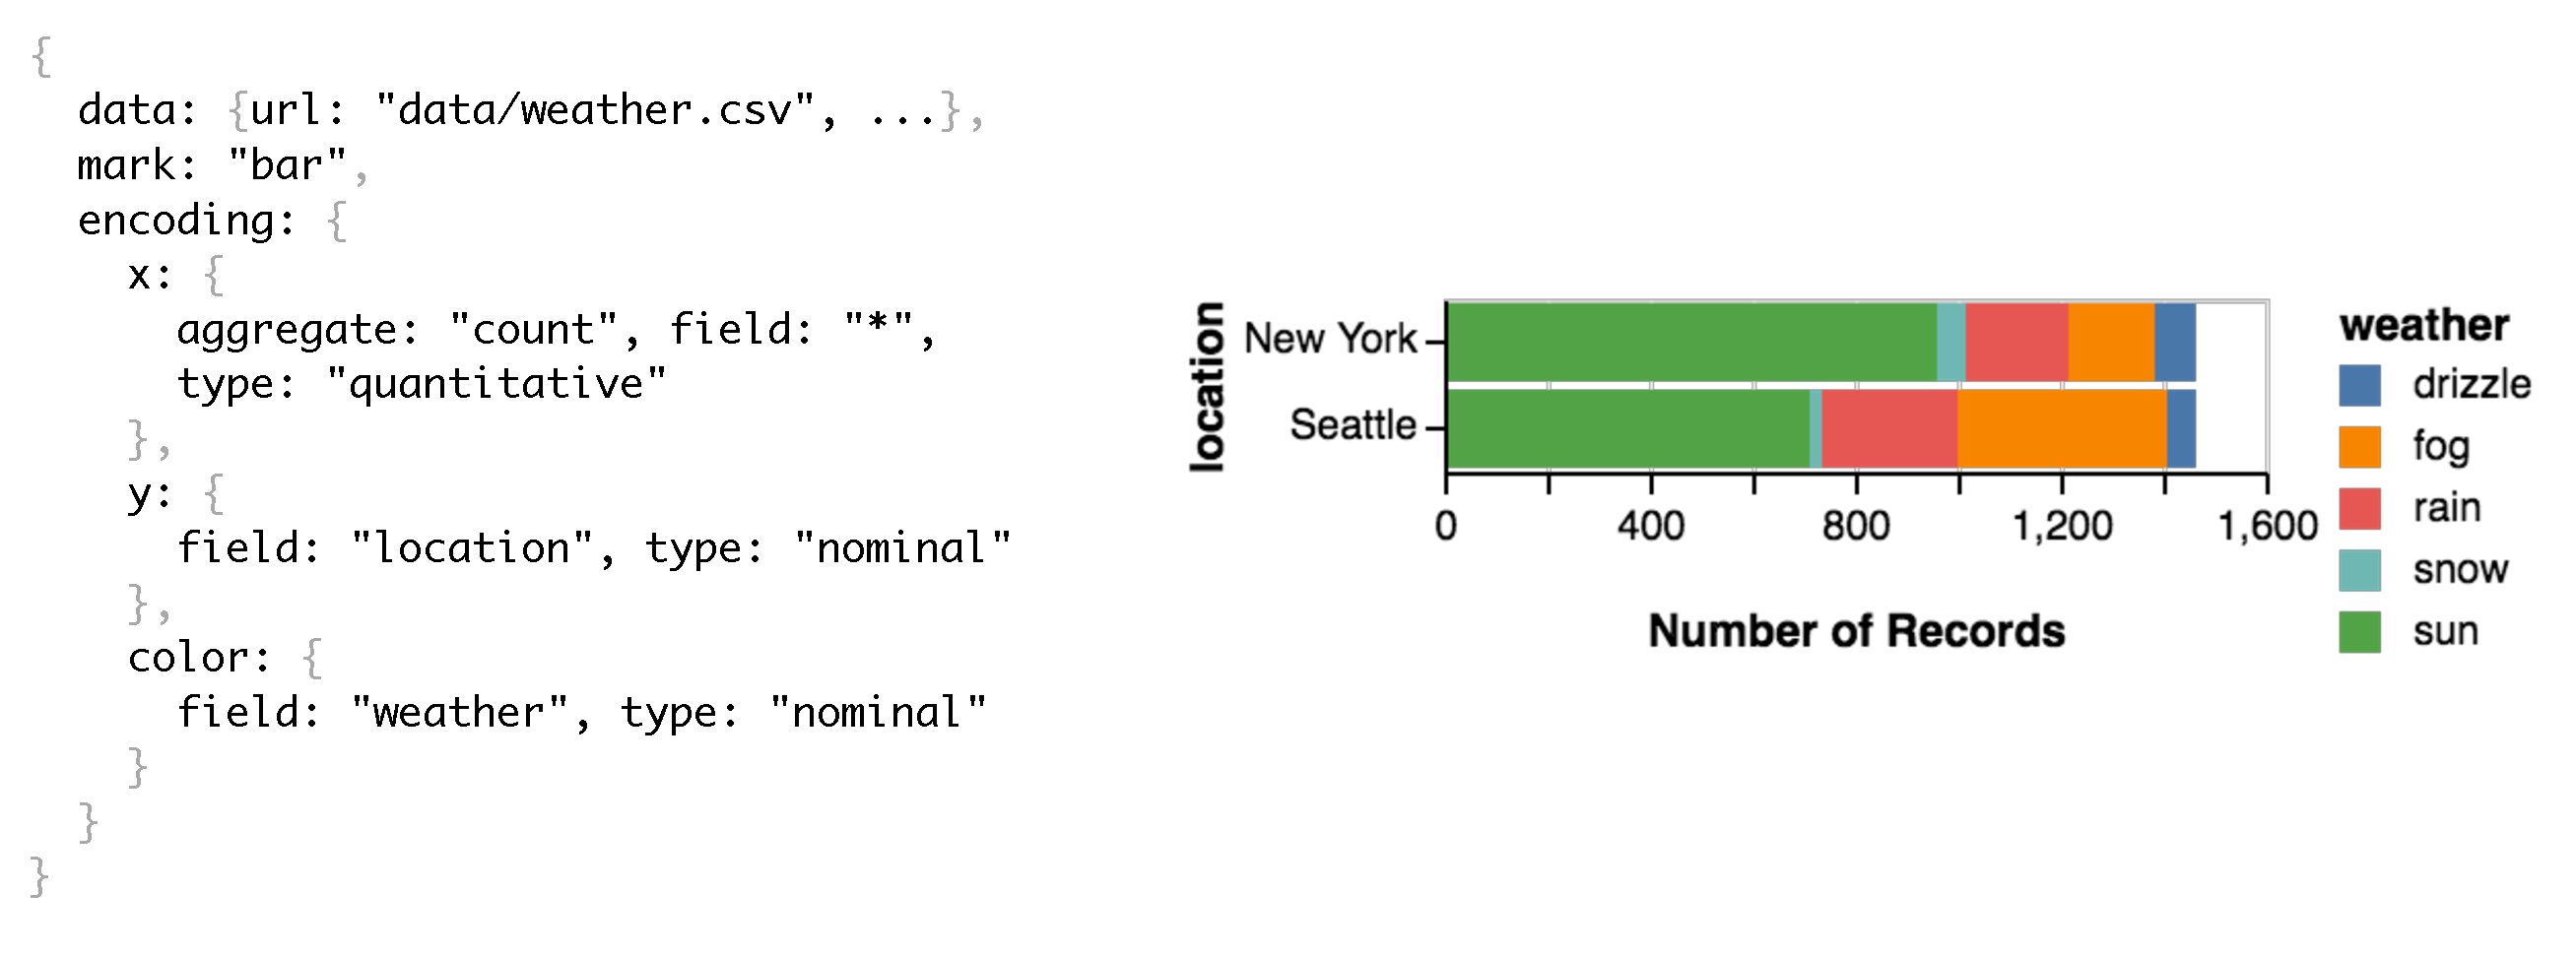
\includegraphics[width=\textwidth]{unit-3}
  \caption{A \emph{stacked} bar chart that sums the various weather types by
  location.}
  \label{fig:unit3}
\end{figure}

\newpage
\section{View Composition Algebra}

Given multiple \emph{unit} specifications, \emph{composite} views can be
constructed using the following operators. Each operator provides default
strategies to \emph{resolve} scales, axes, and legends across views. A user can
choose to override these default behaviors by specifying tuples of the form
\emph{(channel, scale$|$axis$|$legend, union$|$independent)}. We use \emph{view}
to refer to any Vega-Lite specification, be it a \emph{unit} or \emph{composite}
specification.

\subsection{Layer}

\centerline{
  \emph{layer([$unit_1$, $unit_2$, ...], resolve)}
}

The \emph{layer} operator produces a view in which subsequent charts are plotted
on top of each other. To produce coherent and comparable layers, we share scales
(if their types match) and merge guides by default. For example, we compute the
union of the data domains for the \emph{x} or \emph{y} channel, for which we
then generate a single scale. However, Vega-Lite can not enforce that a unioned
domain is \emph{semantically} meaningful. To prohibit layering of composite
views with incongruent internal structures, the \emph{layer} operator restricts
its operands to be \emph{unit} views.

\begin{figure*}[h!]
  \centering
  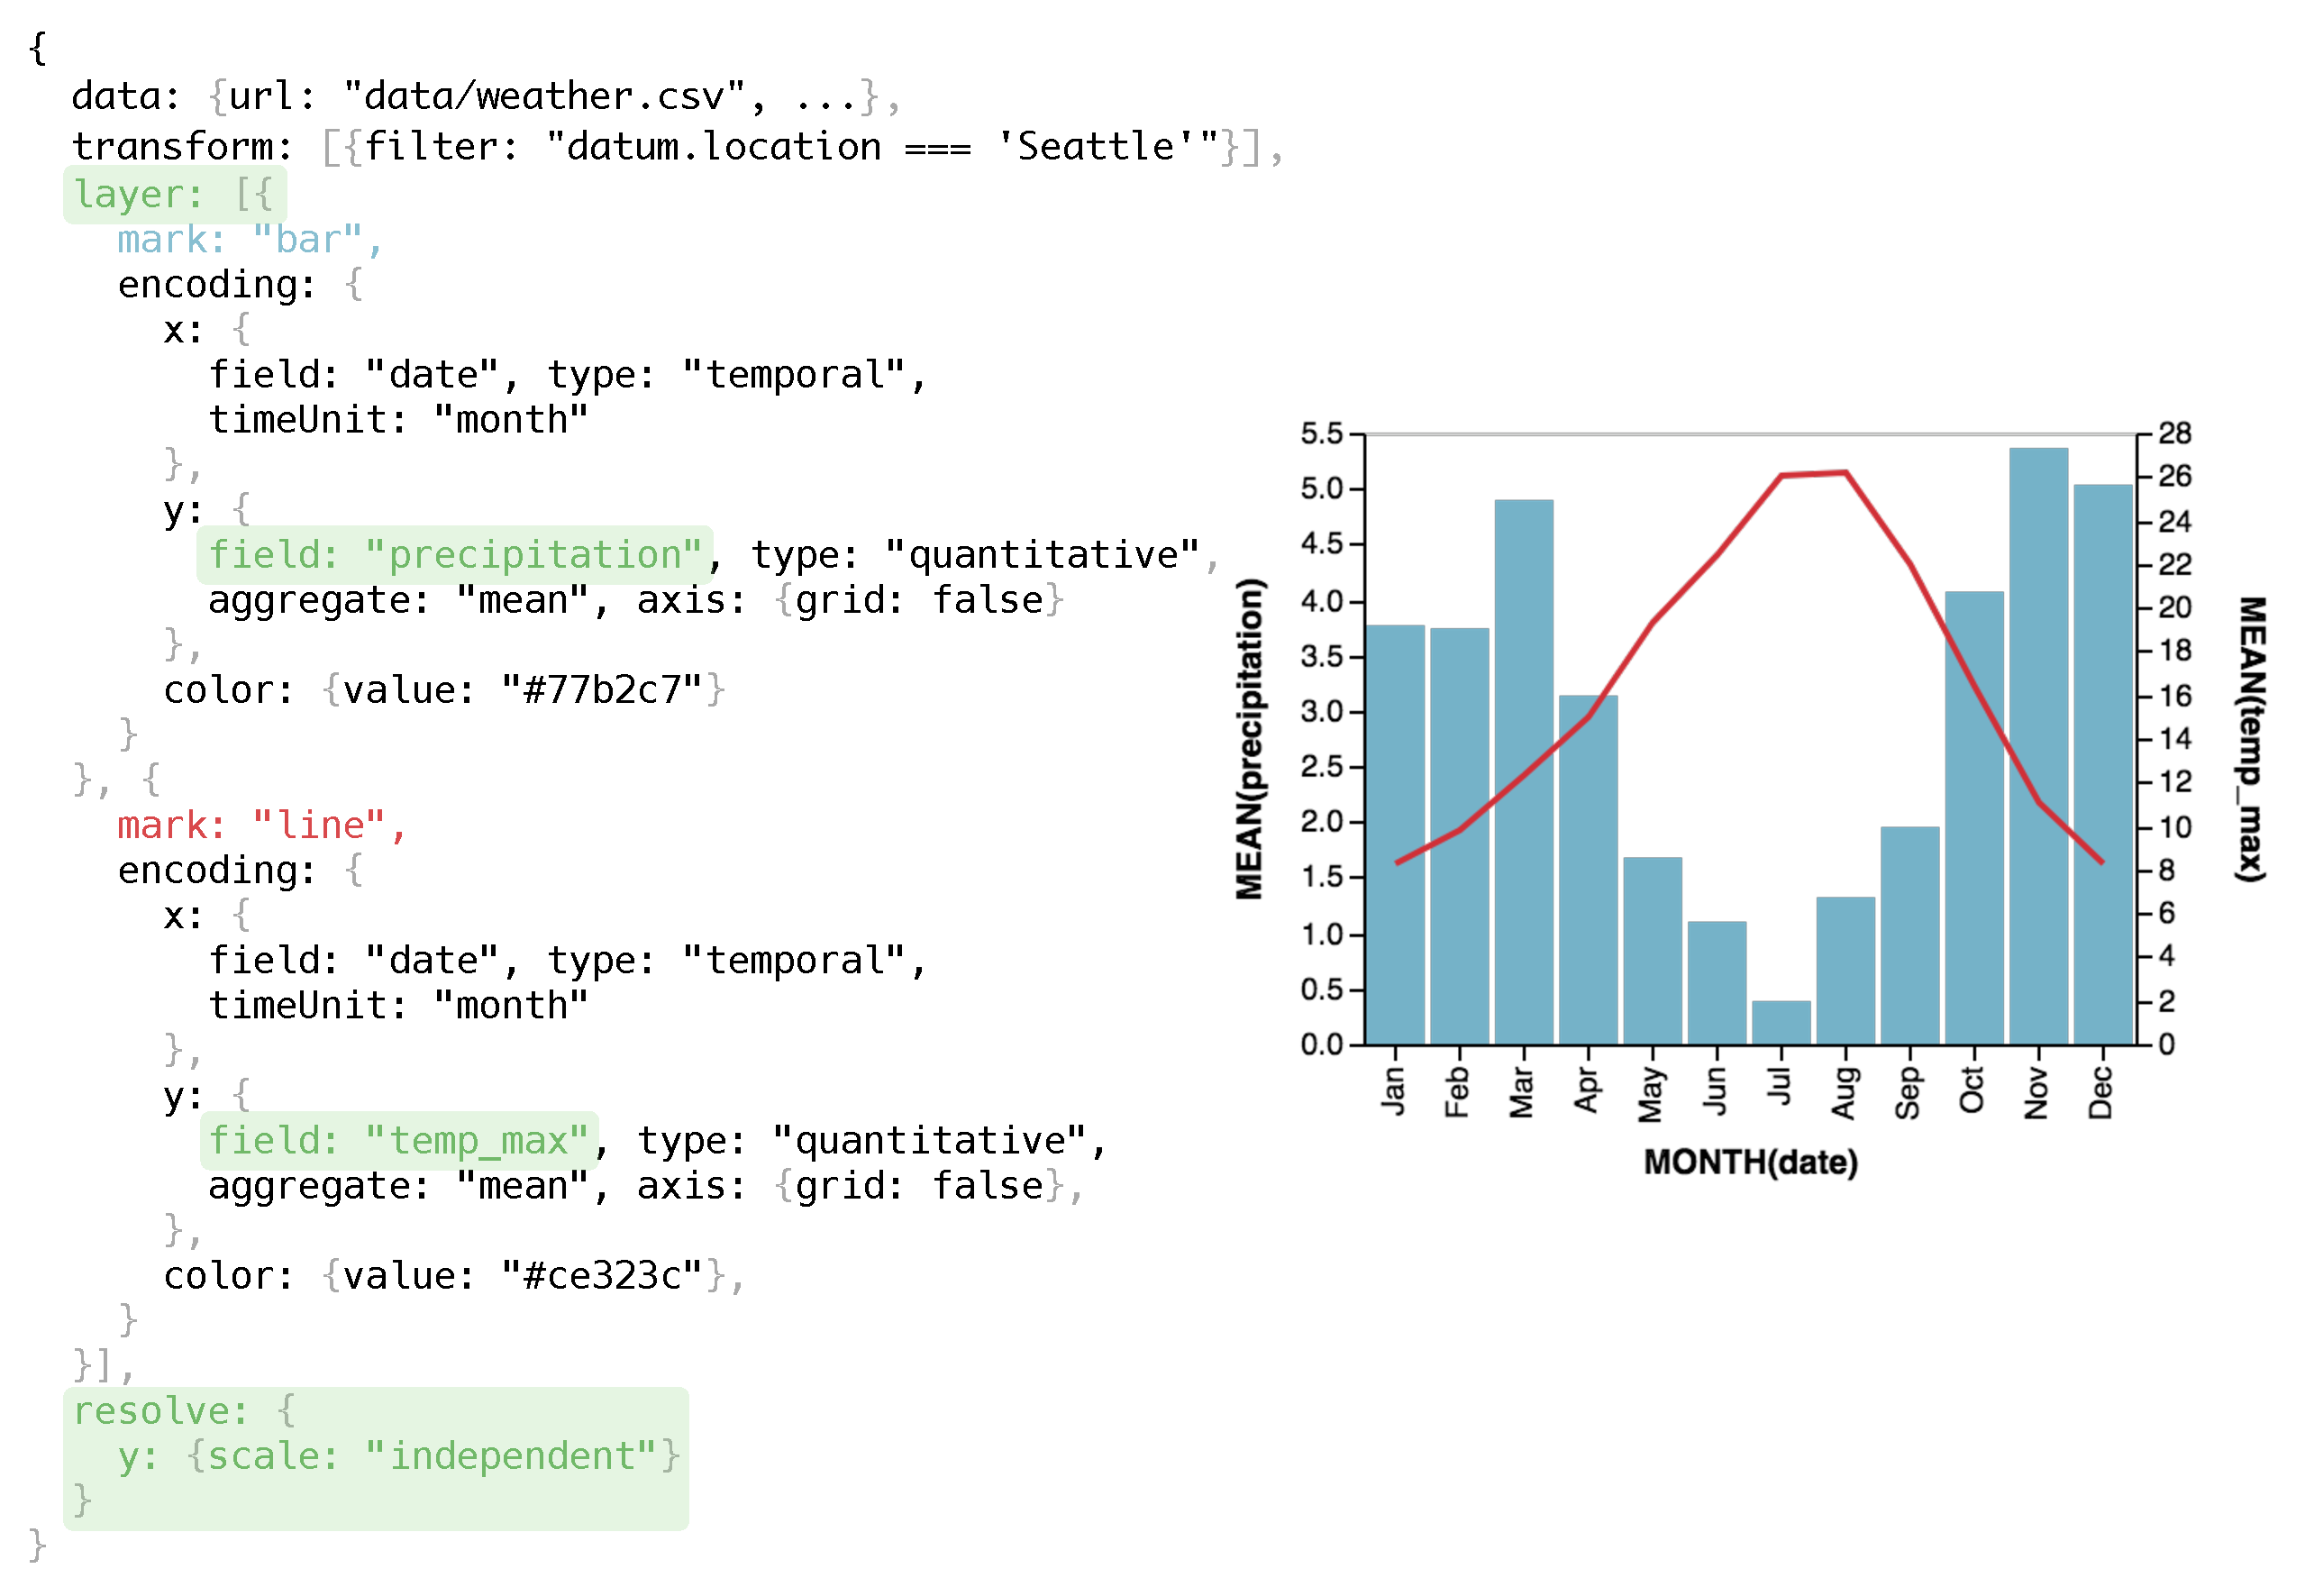
\includegraphics[width=\columnwidth]{layer}
  \caption{A dual axis chart that \emph{layers} a line for the monthly mean
  temperature on top of bars for monthly mean precipitation. Each layer uses an
  \emph{independent} y-scale.}
  \label{fig:layer}
\end{figure*}

\subsection{Concatenation}

\centerline{
  \emph{hconcat([$view_1$, $view_2$, ...], resolve)}
}
\centerline{
  \emph{vconcat([$view_1$, $view_2$, ...], resolve)}
}

The \emph{hconcat} and \emph{vconcat} operators place views side-by-side
horizontally or vertically, respectively. If aligned spatial channels have
matching data fields (e.g., the \emph{y} channels in an \emph{hconcat} use the
same field), a shared scale and axis are used. Axis composition facilitates
comparison across views and optimizes the underlying implementation.

\begin{figure*}[h!]
  \centering
  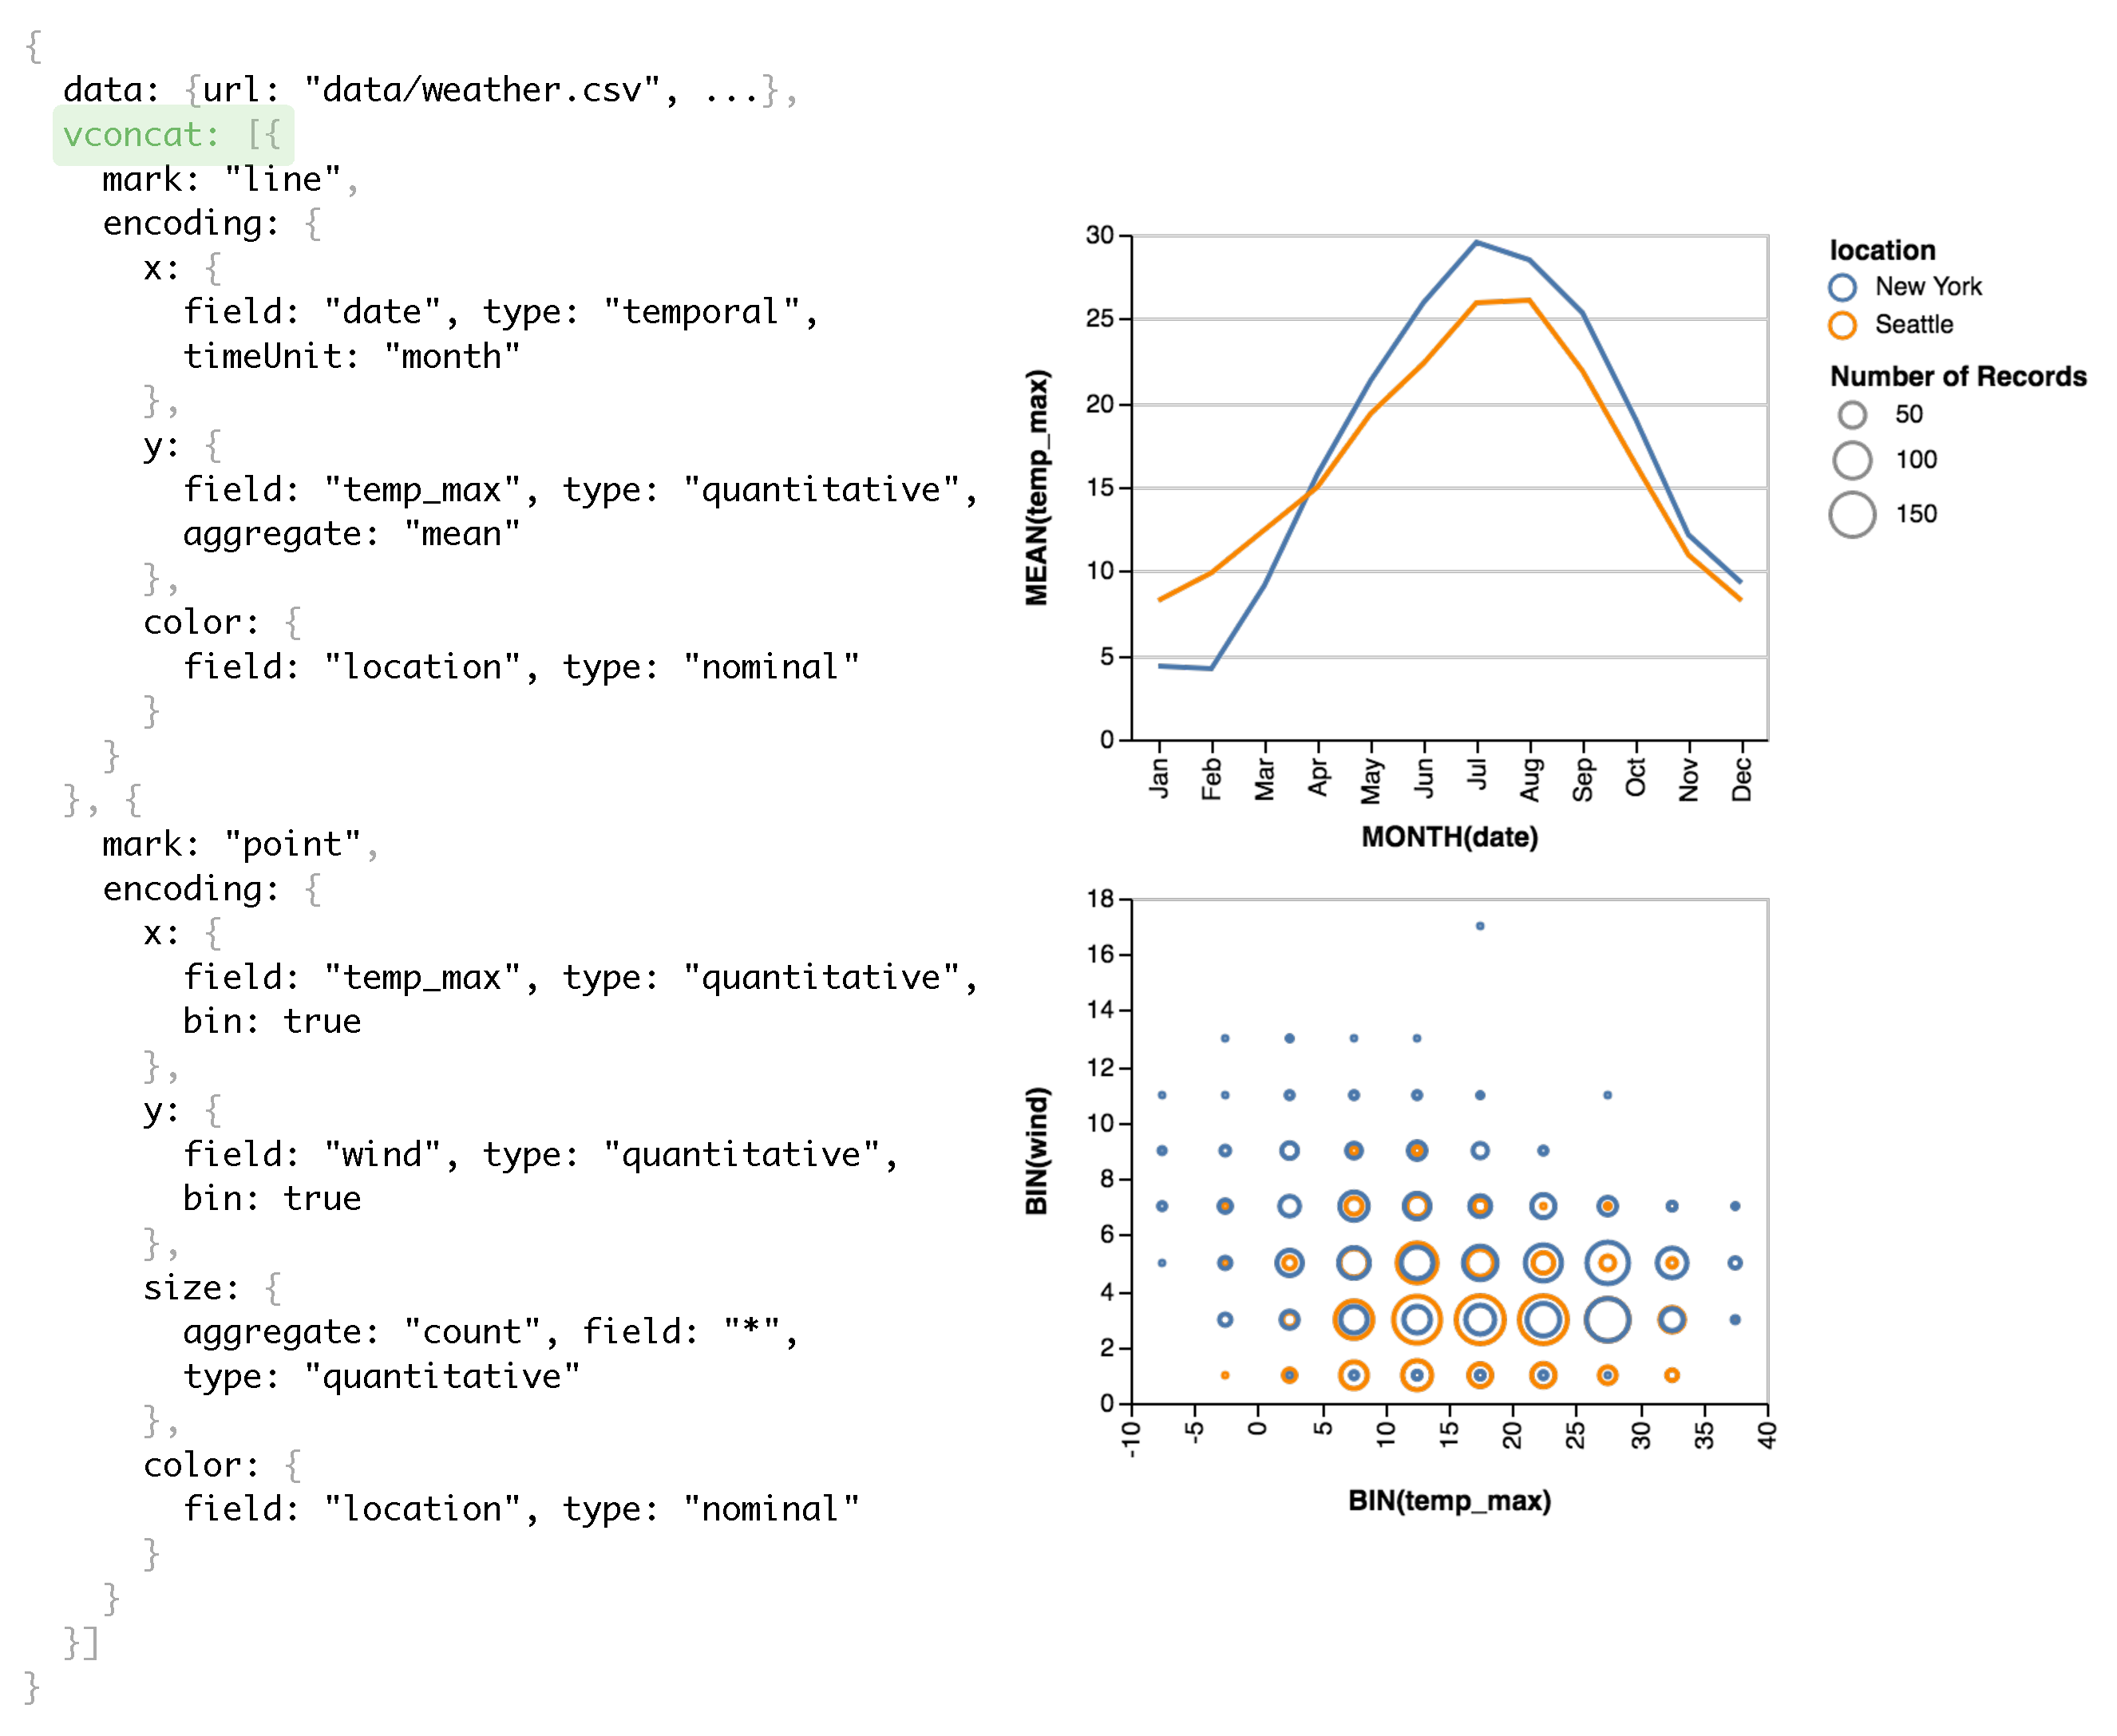
\includegraphics[width=\columnwidth]{concat}
  \caption{The \cref{fig:unit1,fig:unit2} unit specifications
  \emph{concatenated} vertically; scales and guides for each
  plot are independent by default.}
  \label{fig:concat}
\end{figure*}

\subsection{Facet}

\centerline{
  \emph{facet(channel, data, field, view, scale, axis, resolve)}
}


The \emph{facet} operator produces a trellis plot~\cite{becker:trellis} by
subsetting the \emph{data} by the distinct values of a \emph{field}. The
\emph{view} specification provides a template for the sub-plots, and inherits
the backing \emph{data} for each partition from the operator. The \emph{channel}
indicates if sub-plots should be laid out vertically (\emph{row}) or
horizontally (\emph{column}), and the \emph{scale} and \emph{axis} parameters
enable further customization of sub-plot layout and labeling.

To facilitate comparison, scales and guides for quantitative fields are shared
by default. This ensures that each facet visualizes the same data domain.
However, for ordinal scales we generate independent scales by default to avoid
unnecessary inclusion of empty categories, akin to Polaris' \emph{nest}
operator. When faceting by fiscal quarter and visualizing per-month data in
each cell, one likely wishes to see three months per quarter, not twelve
months of which nine are empty.

\begin{figure*}[h!]
  \centering
  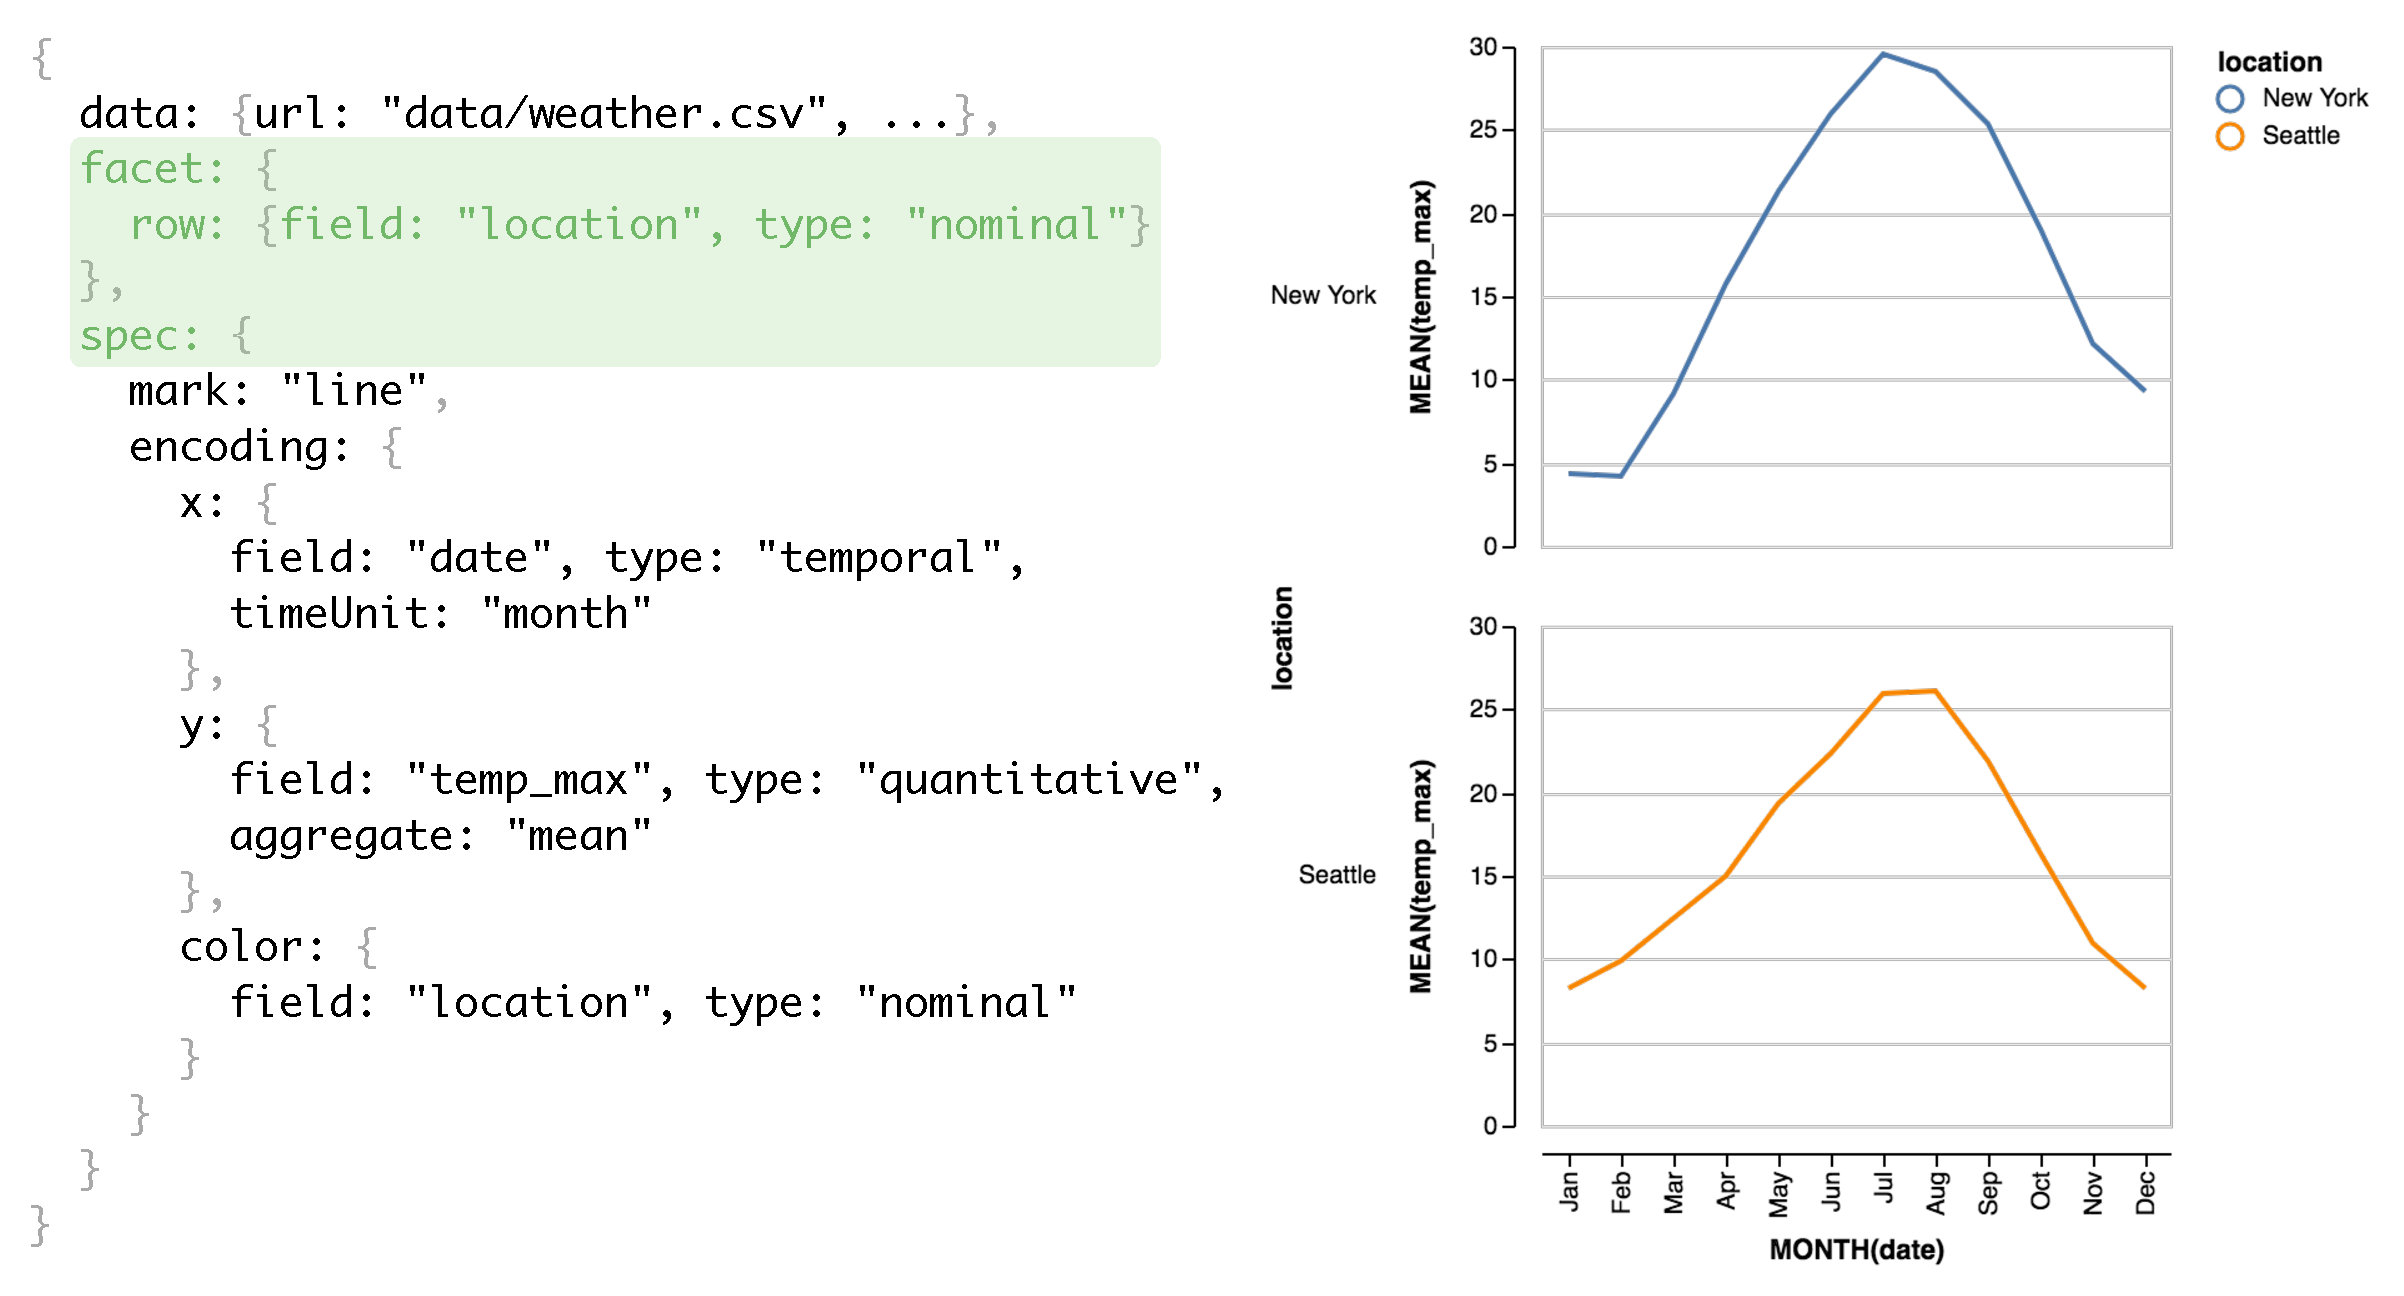
\includegraphics[width=\columnwidth]{facet}
  \caption{The line chart from \cref{fig:unit1} \emph{faceted}
  vertically by location; the x-axis is shared, and the underlying scale domains
  unioned, to facilitate easier comparison.}
  \label{fig:facet}
\end{figure*}

\subsection{Repeat}

\centerline{
  \emph{repeat(channel, values, scale, axis, view, resolve)}
}

The \emph{repeat} operator generates one plot for each entry in a list of
\emph{values}. The \emph{view} specification provides a template for the
sub-plots, and inherits the full backing dataset. Encodings within the
repeated \emph{view} specification can refer to this provided \emph{value} to
parameterize the plot\footnote{As the \emph{repeat} operator requires
parameterization of the inner view, it is not strictly algebraic. It is
possible to achieve algebraic ``purity'' via explicit repeated concatenation
or by reformulating the repeat operator (e.g., by including rewrite rules that
apply to the inner view specification). However, we believe the current syntax
to be more usable and concise than these alternatives.}. As with \emph{facet},
the \emph{channel} indicates if plots should divide by \emph{row} or
\emph{column}, with further customization possible via the \emph{scale} and
\emph{axis} components. By default, scales and axes are independent, but
legends are shared when data fields coincide.

\begin{figure*}[h!]
  \centering
  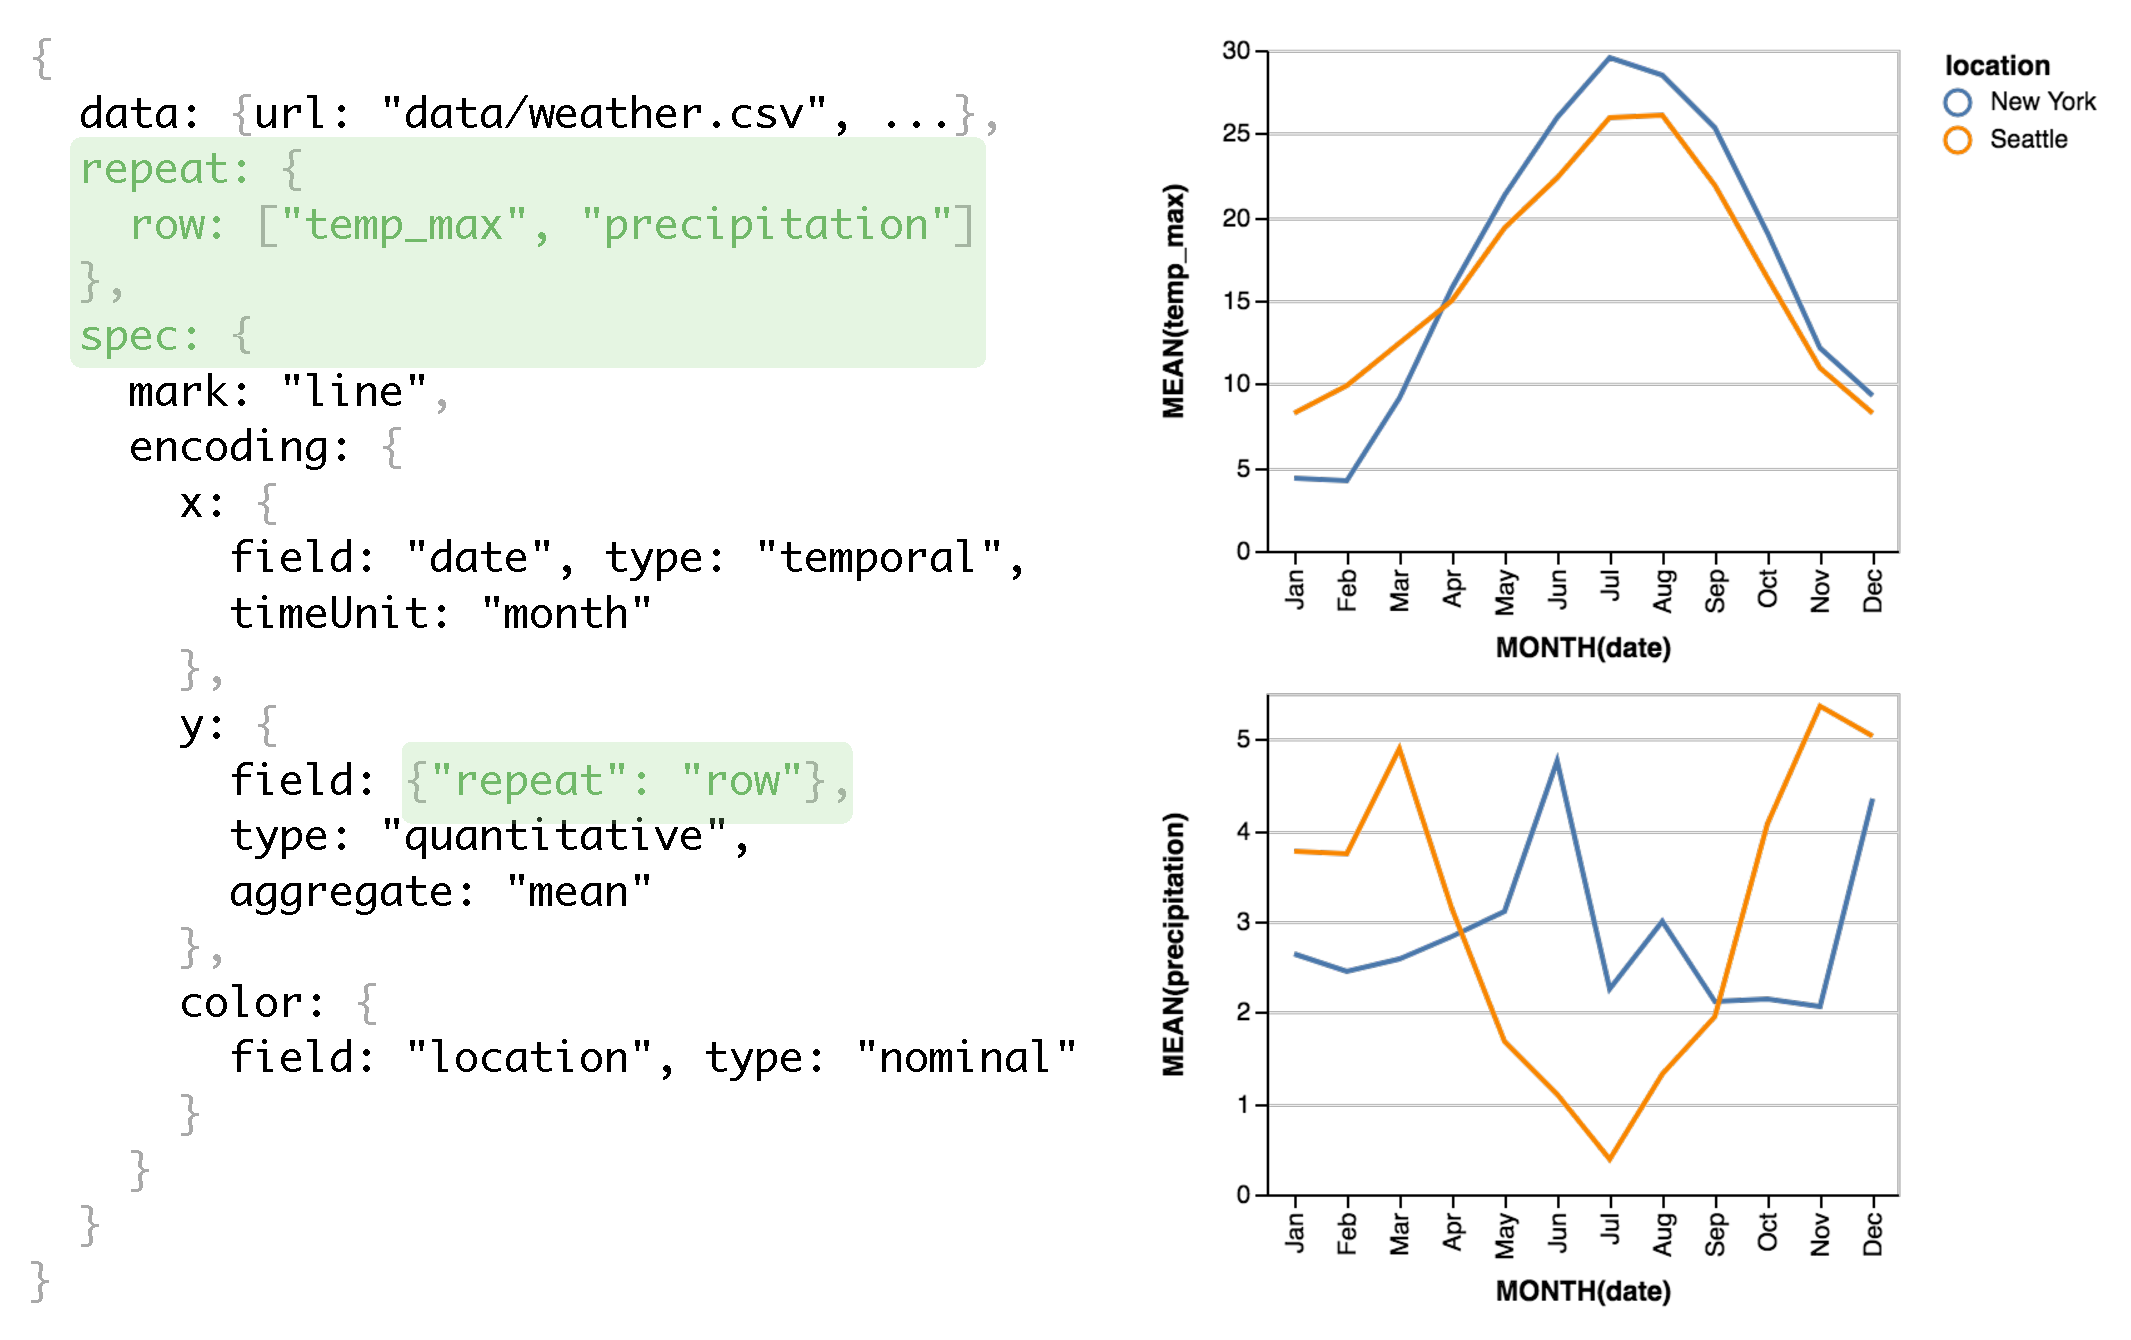
\includegraphics[width=\columnwidth]{repeat}
  \caption{\emph{Repetition} of different measures across rows; the y-channel
  references the \texttt{row} template parameter to vary the encoding.}
  \label{fig:repeat}
\end{figure*}

\subsection{Dashboards and Nested Views}

These view composition operators form an algebra: the output of one operator can
serve as input to a subsequent operator. As a result, complex dashboards and
nested views can be concisely specified. For instance, a layer of two unit views
might be repeated, and then concatenated with a different unit view. The one
exception is the \emph{layer} operator, which, as previously noted, only accepts
unit views to ensure consistent plots. For concision, two dimensional faceted or
repeated layouts can be achieved by applying the operators to the \emph{row} and
\emph{column} channels simultaneously. When faceting a composite view, only the
dataset targeted by the operator is partitioned; any other datasets specified in
sub-views are replicated.